
\chapter{Semi-inclusive deep inelastic scattering and the $A_{UT}$ asymmetry}
\section{Kinematics, frame and factorization}
\noindent As anticipated, we study the semi-inclusive lepton-nucleon process described by
\begin{equation}
    e(l)+N(P,S) \longrightarrow e(l')+h(P_h)+X .
\end{equation}
Defining the space-like momentum of the virtual photon as $q^\mu=l^\mu-l'^\mu$, the usual SIDIS kinematical variables are given by
\begin{equation}
    \begin{aligned}
        x_B=\frac{Q^2}{2P\cdot q},\qquad y=\frac{P\cdot q}{P\cdot l},\qquad z_h=\frac{P\cdot P_h}{P\cdot q}.
    \end{aligned}
\end{equation}
For reasons that will hopefully be clear soon, the initial factorization of the cross section is conveniently derived in a frame in which the nucleon and hadron momenta are collinear along the $z$ axis. As typical in a pQCD calculation, we neglect all lepton and hadron masses, since we are interested in the high-energy scattering limit. This means that both the nucleon and the outgoing hadron momenta are approximately light-like vectors, i.e. $P^2=P_h^2\approx0$. It is therefore natural to introduce transverse projectors that specify the components of any 4-vector that is transverse to both the nucleon and the hadron momenta. The projector in this frame reads
\begin{equation}
    g_T^{\mu\nu}=g^{\mu\nu}-\frac{1}{P\cdot P_h}(P^\mu P_h^\nu+P^\nu P_h^\mu).
\end{equation}
It is also useful to introduce a set of auxiliary light-cone vectors $n^\mu=\frac{2x_B}{z_hQ^2}P_h^\mu$ with $n^2=0$ and $n\cdot P=1$, along with $m^\mu=\frac{2x_B}{z_hQ^2}P^\mu$ with $m^2=0$ and $m\cdot P_h=1$. The transverse projector can then be cast in the following equivalent form
\begin{equation}
    g^{\mu\nu}_T=g^{\mu\nu}-n^\mu P^\nu - n^\nu P^\mu=g^{\mu\nu}-m^\mu P_h^\nu - m^\nu P_h^\mu.
\end{equation}
With this conventions, a transverse vector will be simply denoted as $a_T^\mu=g^{\mu\nu}_Ta_\nu$. In this frame, we have the following parametrization of the four-vectors $a^\mu=(a^0,\vec a)$ \cite{}:
\begin{equation}
    \begin{aligned}
        P^\mu&=\Big(\frac{Q}{2x_B},0,0,\frac{Q}{2x_B}\Big),\\
        P_h^\mu&=\Big(\frac{z_hQ}{2},0,0,-\frac{z_hQ}{2}\Big),\\
        q^\mu&=\Big(\frac{Q_T^2}{2Q},Q_T\cos\phi_q,Q_T\sin\phi_q,-Q+\frac{Q_T^2}{2Q}\Big),\\
        q^\mu_T&=\Big(0,Q_T\cos\phi_q,Q_T\sin\phi_q,0\Big),\\
    \end{aligned}
\end{equation}
where $Q_T=\sqrt{-q_T^2}$. 
%It is often useful to express the virtual photon momentum as a combination of the hadronic momenta
%\begin{equation}
%    q^\mu = -x_B(1-\chi^2_T)P^\mu+\frac{1}{z_h}P_h^\mu + q_T^\mu
%\end{equation}
%where for convenience we introduced the positive parameter $\chi_T^2\equiv Q_T^2/Q^2$.
It is therefore clear that in a frame where the nucleon and the outgoing hadron are collinear, a light-cone decomposition is possible and the meaning of "transverse" with respect to the hadron momenta is clearly understood. The 4-dimensional space is hence partitioned in a "plus" direction, a "minus" direction and a 2-dimensional transverse space. For a generic 4-vector $a^\mu$, the following decomposition holds
\begin{equation}
    a^\mu = (a\cdot n)P^\mu + (a \cdot P)n^\mu+a_T^\mu=(a\cdot m)P_h^\mu + (a \cdot P_h)m^\mu+a_T^\mu.
\end{equation}  
By denoting as $k^\mu$ the momentum of the parton coming from the nucleon, and $p^\mu$ the fragmenting partonic momentum,  we have
\begin{equation}
    \begin{aligned}
        k^\mu &= xP^\mu + k_T^\mu+(k\cdot P)n^\mu\approx xP^\mu + k_T^\mu,\\
        p^\mu &= \frac{1}{z}P_h^\mu + p_T^\mu+(p\cdot P_h)m^\mu\approx \frac{1}{z}P_h^\mu + p_T^\mu,
    \end{aligned}
\end{equation}
where, as typical, we neglected contributions of order two or higher in the transverse momenta. Note that this approximation is consistent with the application of the collinear twist-3 formalism, since we will need only linear terms in $k_T$ or $p_T$ to fully derive a factorized spin-dependent cross section.

\noindent The relevant Feynman diagrams for SIDIS at LO are given in Fig.~\ref{fig:amplitudes SIDIS LO}. The lower and upper colored blobs are nothing else but non-perturbative matrix elements introduced in the previous chapter. For a direct generalization to NLO, we isolate the hard-scattering amplitude $\hat{\mathcal{M}}$ of the partonic subprocess with the virtual photon.
\begin{figure}
    \centering
    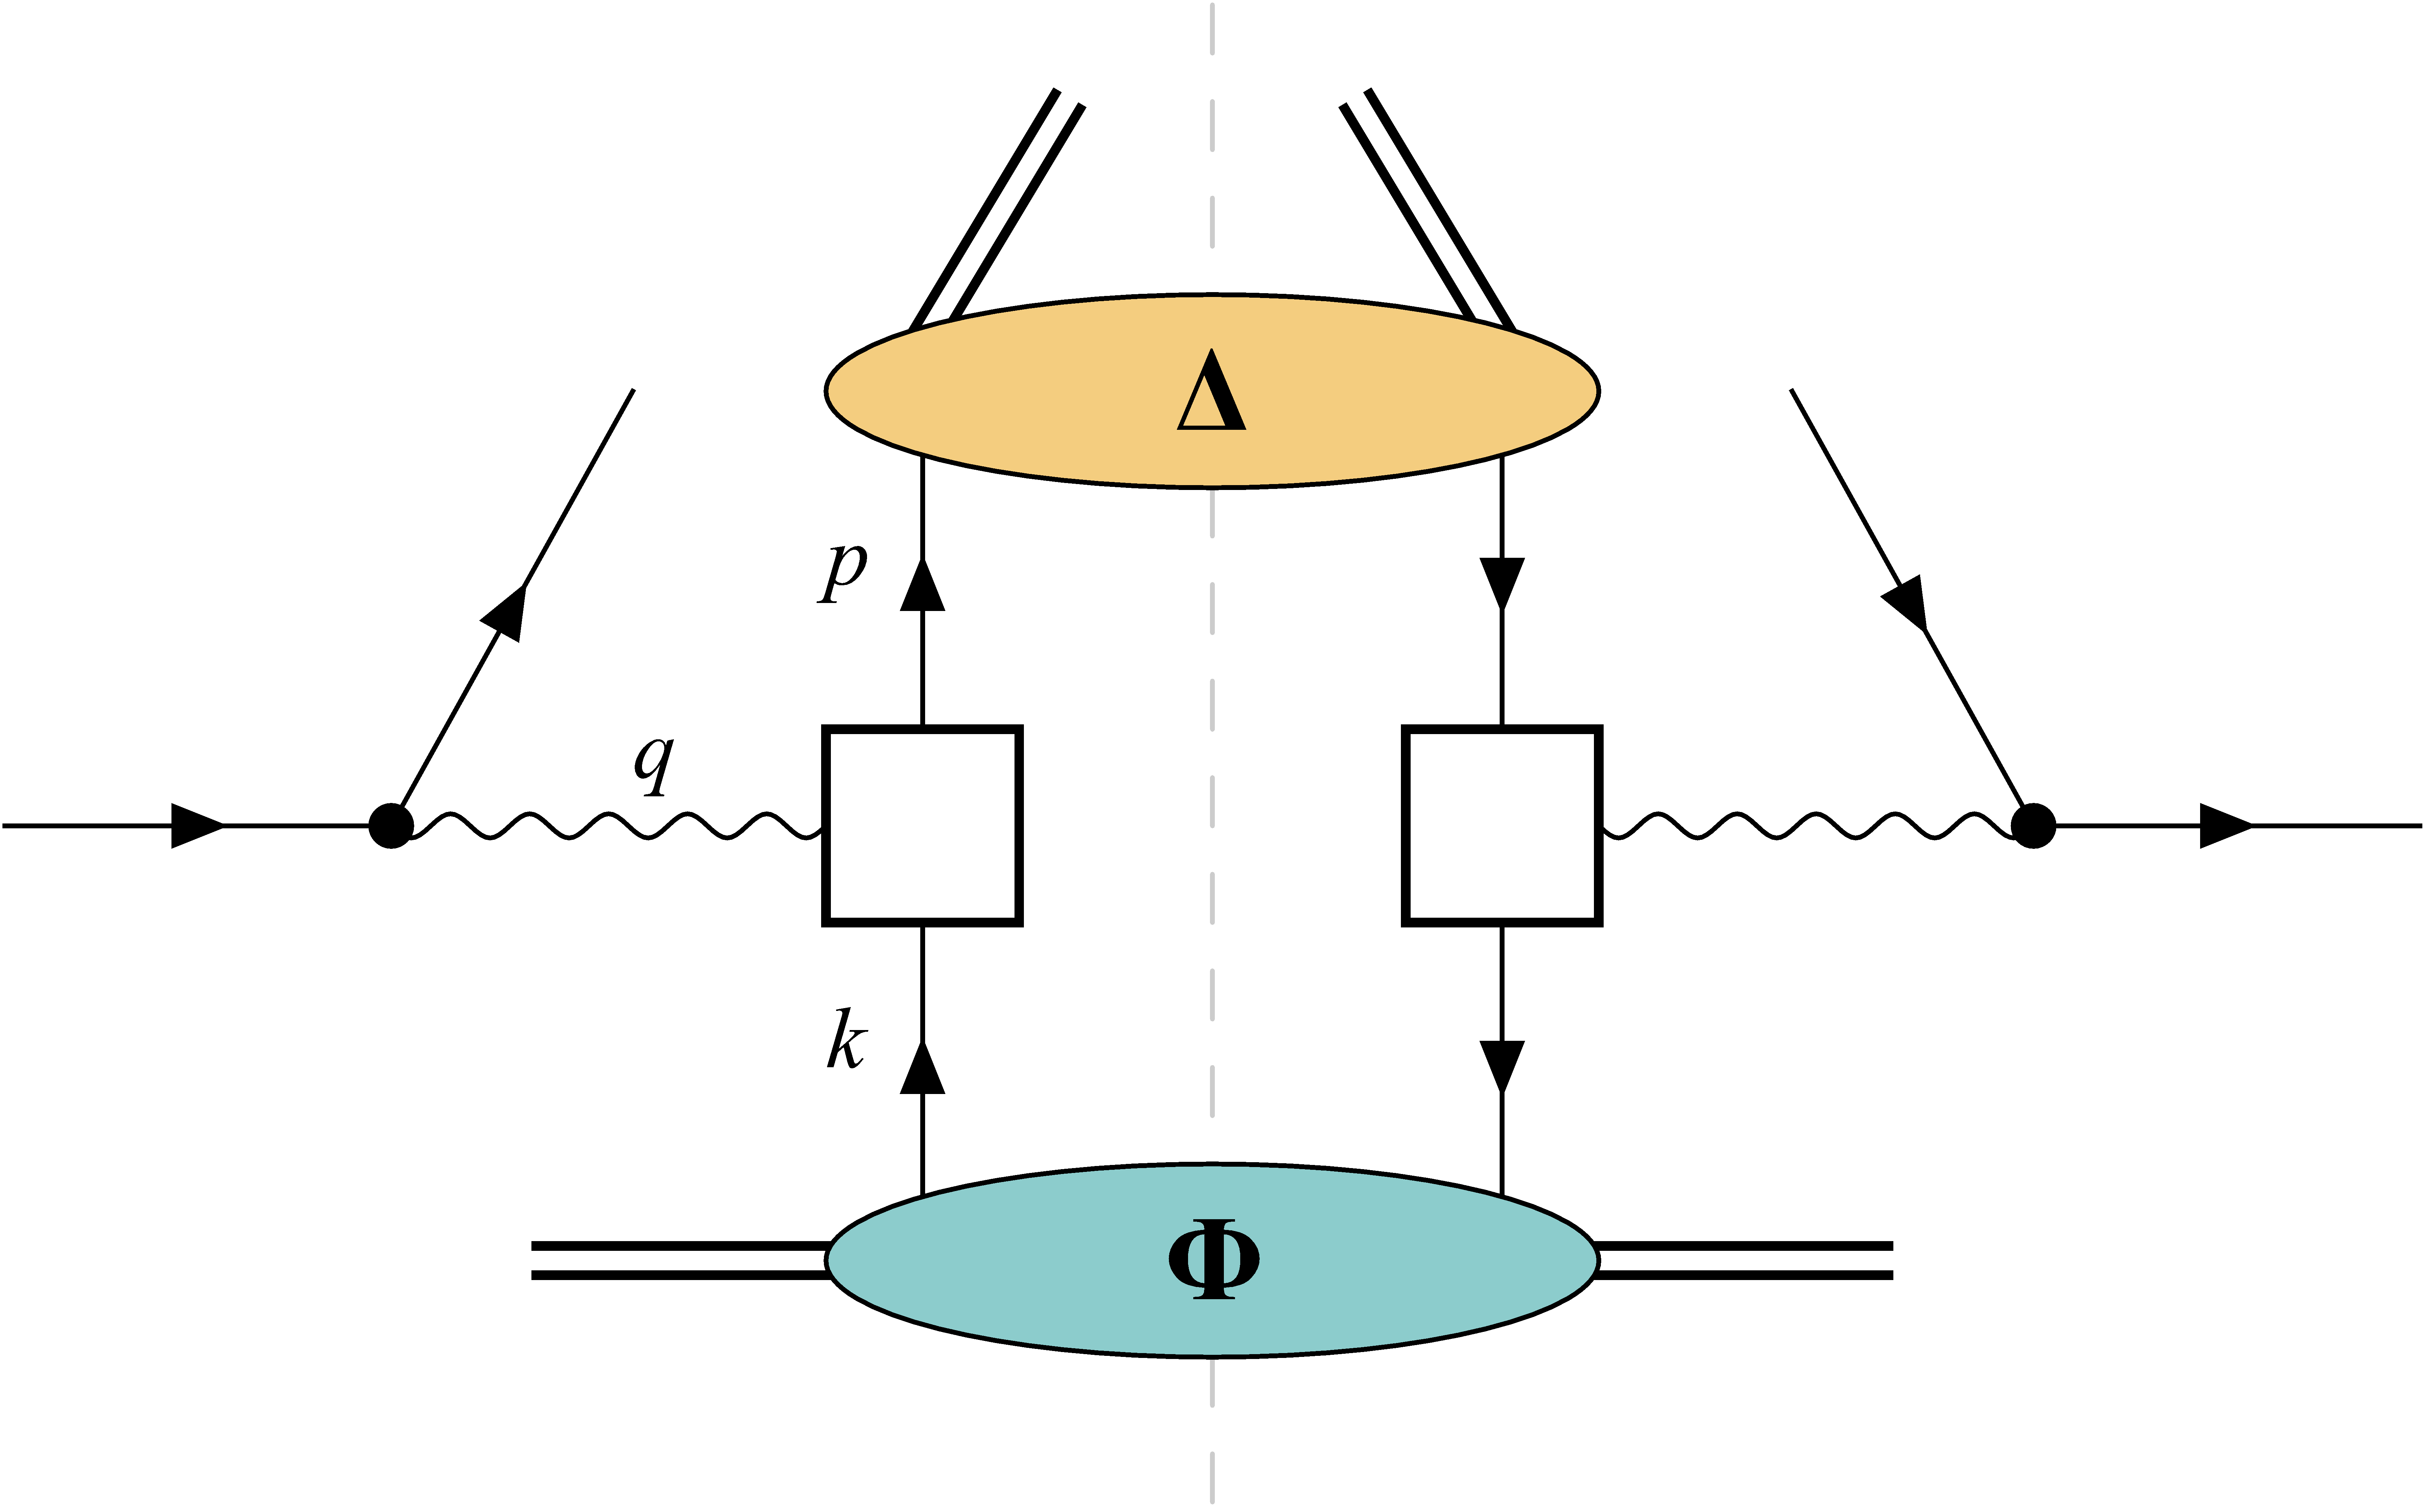
\includegraphics[width=0.5\linewidth]{fig/SIDIS q2q v2.png}
    \caption{Caption}
    \label{fig:amplitudes SIDIS LO}
\end{figure}
\noindent The differential cross section is then obtained by employing QCD and QED Feynman rules and hadronic matrix elements \cite{Weinberg_1995}. For direct generalization to a NLO case, we perform the calculation in dimensional regularization in $d=4-2\epsilon$ dimensions. We obtain
\begin{equation}\label{eq:dsigma general master formula}
\begin{aligned}
        \dd \sigma = &\frac{1}{F}\frac{\dd ^{d-1}\boldsymbol l'}{(2\pi)^{d-1} 2E'}\frac{\dd^{d-1}\boldsymbol {P_h}}{(2\pi)^{d-1} 2E_h}\frac{(4\pi)^2\alpha_{em}^2}{Q^4}L^{\mu\nu} \,W_{\mu\nu},
\end{aligned}
\end{equation}
with the leptonic tensor $L^{\mu\nu}$ defined as
\begin{equation}
            L^{\mu\nu}=\frac{1}{2}\Tr[(1+\lambda_e\gamma_5)\slashed{l}\gamma^\nu \slashed{l}'\gamma^\mu],
\end{equation}
where $\lambda_e$ denotes the helicity of the incoming lepton. The hadronic tensor $W_{\mu\nu}$, evidently, assumes different forms depending on the reaction channel. We derive 
\begin{equation}
\begin{aligned}
        W_{\mu\nu}^{q \to q}&=\sum_a  e_a^2\int\dd^d k\int \dd^{d}p\,\delta^{(d)}(q+k-p)\Tr[\hat{\mathcal{M}}_\mu^{q\to q} \Phi^a\hat{\bar{\mathcal{M}}}_\nu^{q\to q}\Delta^a]\\
        W_{\mu\nu}^{gq \to q}&=\sum_a e_a^2\int\dd^d k\int \dd^{d}p\int \dd^{d}k'\,\delta^{(d)}(q+k-p)\Tr[\frac{\hat{\mathcal{M}}_{\mu\sigma}^{gq\to q}}{g_S T^\alpha} \Phi_A^{\sigma,a}\hat{\bar{\mathcal{M}}}_\nu^{q\to q}\Delta^a]\\
        W_{\mu\nu}^{q \to gq}&= \sum_a e_a^2\int\dd^d k\int \dd^{d}p\int \dd^{d}p'\,\delta^{(d)}(q+k-p)\Tr[\frac{\hat{\mathcal{M}}_{\mu\sigma}^{q\to g q}}{g_S T^\alpha} \Phi^{a}\hat{\bar{\mathcal{M}}}_\nu^{q\to q}\Delta_A^{\sigma,a}]
        \end{aligned}
\end{equation}
with $\Phi^a, \Delta^a,\Phi_A^{\sigma,a}\Delta_A^{\sigma,a}$ the correlators introduced in the previous chapter, but in their fully-unintegrated versions. Here, the $\sum_a$ really just means a sum over quarks and anti-quarks flavours ($a=q,\bar{q}$). All momenta are now decomposed through the light-cone decomposition introduced before. Performing the (trivial) integrations over $\dd (k \cdot P)$ and $\dd (p\cdot P_h)$, one sees that the integral measures and the delta function arrange in the following way
\begin{equation}
    \begin{aligned}
        \dd^d k \,\dd^d p &\,\delta^{(d)}(q+k-p) \sim\dd x\, \dd^{d-2}k_T\, \frac{\dd z}{z^2}\, \dd^{d-2}p_T\, \\
        & \times\frac{2x_B z_h}{Q^2}\delta(x-x_B(1-\chi_T^2))\delta(z-z_h)\delta^{(d-2)}(\vec q_T+\vec k_T-\vec p_T).        
    \end{aligned}
\end{equation}
We stress that the separation of the delta function in such a way makes sense only in a frame where the nucleon and the hadron are collinear, i.e. the $PP_h$ frame used so far. In this case, the transverse vectors are indeed 2-dimensional and this kind of $(+,-,T)$ separation makes sense.

Our goal is to study the differential cross section integrated over transverse momentum of the observed hadron. However, in a collinear frame such as the one used so far, the momentum $P_h$ is fixed and it has no transverse component by construction. A possible approach would be to integrate over the transverse momentum $q_T$ of the virtual photon. However, the leptonic tensor $L^{\mu\nu}$ clearly will depend on this transverse momentum, making a clean separation between leptonic and hadronic parts impossible. A common procedure is then to change frame in such a way that this separation is possible \cite{meng_semi-inclusive_1992,mulders_complete_1996, bacchetta_semi-inclusive_2007}. \\
ADD HERE DISCUSSION OF BOER03\\
It turns out that the Breit frame in which the virtual photon and the nucleon are collinear is an appropriate choice. In this new frame, the photon momentum doesn't have a temporal component (which is possible since in SIDIS $q^\mu$ is always a space-like vector). The hadron momentum  now acquires a perpendicular component. We then construct the Lorentz transformation from the $PP_h$ frame to the Breit frame. It turns out to be
\begin{equation}
    \Lambda^\mu_\nu=\mqty(1+\frac{Q_T^2}{2Q^2} & -\frac{Q_T}{Q}\cos\phi_q & -\frac{Q_T}{Q}\sin\phi_q & -\frac{Q_T^2}{2Q^2}\\
    -\frac{Q_T}{Q}\cos\phi_q  & 1 & 0 & \frac{Q_T}{Q}\cos\phi_q \\
    -\frac{Q_T}{Q}\sin\phi_q  & 0 & 1 & \frac{Q_T}{Q}\sin\phi_q \\
    \frac{Q_T^2}{2Q^2} & -\frac{Q_T}{Q}\cos\phi_q & -\frac{Q_T}{Q}\sin\phi_q & 1-\frac{Q_T^2}{2Q^2}
    )
\end{equation}
We note that this transformation satisfies the usual Lorentz transformation properties $\det\Lambda=1$ and $\Lambda^T g \Lambda=g$. In this frame, the momenta read
\begin{equation}\label{eq:momenta in BF}
    \begin{aligned}
        P^\mu&=\Big(\frac{Q}{2x_B},0,0,\frac{Q}{2x_B}\Big)\\
        P_h^\mu&=\frac{z_hQ}{2}\Big(1+\chi_T^2,-2\chi_T\cos\phi_q,-2\chi_T\sin\phi_q,-1+\chi_T^2\Big)\\
        q^\mu&=\Big(0,0,0,-Q\Big)\\
        l^\mu&=\frac{Q}{2}\Big(\frac{2-y}{y},\frac{2}{y}\sqrt{1-y}\cos\phi_l, \frac{2}{y}\sqrt{1-y}\sin\phi_l,-1\Big)\\
        l'^\mu&=\frac{Q}{2}\Big(\frac{2-y}{y},\frac{2}{y}\sqrt{1-y}\cos\phi_l, \frac{2}{y}\sqrt{1-y}\sin\phi_l,+1\Big)
    \end{aligned}
\end{equation}
where $\phi_l$ is an azimuthal angle around the $z$-axis \cite{kanazawa_contribution_2013}. A sketch of the lepton and hadron planes, along with the conventions for the different angles is shown in Fig.~\ref{fig:Breit frame}. It turns out that our results are particularly simple when expressed in terms of the difference $\phi_S-\phi_l$, where $\phi_S$ is the azimuthal angle of the transverse spin vector $\boldsymbol{S}_\perp$ of the nucleon. In fact, one can define such angle through the following Lorentz-invariant expression, adhering to the Trento conventions \cite{bacchetta_single-spin_2004}
\begin{equation}
\begin{aligned}
     \sin(\phi_S-\phi_l)=& -\frac{\epsilon_\perp^{\mu\nu}l_\mu S_\nu}{\sqrt{-g^{\mu\nu}_\perp l_\mu l_\nu}}=-\frac{2x_By}{Q^3\sqrt{1-y}}\epsilon^{lPqS}=+\frac{2x_By}{Q^3\sqrt{1-y}}\epsilon^{lPl'S}\\
      \cos(\phi_S-\phi_l)=& -\frac{g_\perp^{\mu\nu}l_\mu S_\nu}{\sqrt{-g^{\mu\nu}_\perp l_\mu l_\nu}}=\frac{y}{Q\sqrt{1-y}}(\text{TO CHECK})
\end{aligned}
\end{equation}
with the transverse Levi-Civita tensor defined as $\epsilon_\perp^{\mu\nu}=\epsilon^{\rho\sigma\mu\nu}P_\rho P_{h\sigma}/(P\cdot P_h)$. We note that the definition of $\phi_S$ is frame independent, as it should be.
\begin{figure}
    \centering
    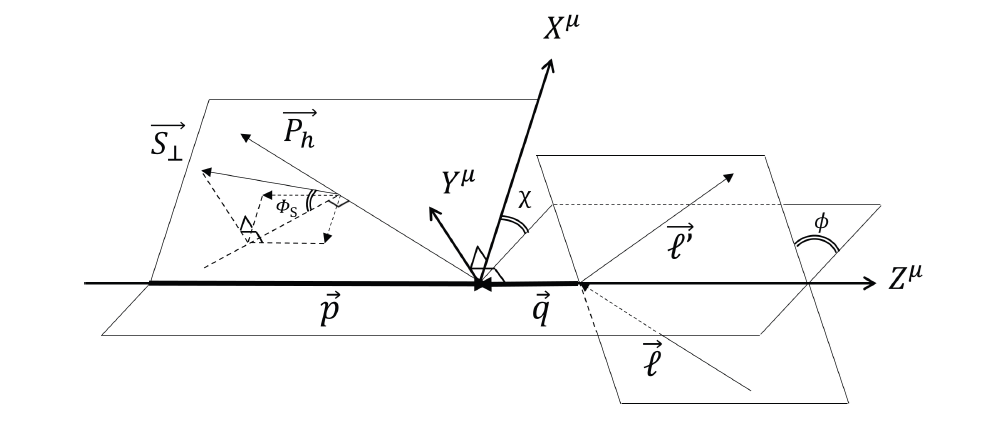
\includegraphics[width=0.7\linewidth]{fig/frame.png}
    \caption{The Breit frame. The virtual photon and the nucleon are collinear along the $z$ axis. In this frame, the hadron momentum $P_h$ acquires a transverse component. The lepton momenta $l,l'$ lie in the lepton plane, which forms an angle $\phi_l$ with respect to the hadron production plane. The transverse spin vector $\boldsymbol{S}_\perp$ of the nucleon forms an angle $\phi_S$ with respect to the lepton plane.}
    \label{fig:Breit frame}
\end{figure}


Also, the partonic momenta now become
\begin{equation}\label{eq:partonic momenta in BF}
    \begin{aligned}
        k^\mu&=xP^\mu+k_T^\mu\eval_{\text{BF}}=x P^\mu+\vec k_\perp^\mu+2x_B\frac{\vec k_\perp^2}{Q^2}P^\mu\\
        p^\mu&=\frac{1}{z}P_h^\mu+p_T^\mu\eval_{\text{BF}}=\frac{1}{z}P_h^\mu+\vec p_\perp^\mu-2x_B\frac{\vec p_\perp^2}{Q^2}P^\mu
    \end{aligned}
\end{equation}
where $P$ and $P_h$ are in the Breit frame, of course. We anticipate that at LO, after integration, the momentum of the detected hadron can be written as
\begin{equation}
    P_h^\mu= z_h(x_BP^\mu+q^\mu)+z_hx_B\frac{(\vec k_\perp - \vec p_\perp)^2}{Q^2}P^\mu+z_h(\vec k_\perp-\vec p_\perp)^\mu.
\end{equation}
Accordingly, one of the light cone vectors remain unchanged $m ^\mu\to m^\mu=\frac{2x_B}{z_hQ^2}P^\mu$ while the other is modified $n^\mu\to n^\mu=\frac{2x_B}{Q^2}(x_BP^\mu+q^\mu)+\mathcal{O}(k_\perp,p_\perp)$. We note the important fact that in one frame transverse 4-momenta are actually just 2-dimensional vectors, but in the Breit frame the perpendicular 4-vector also acquires a component in the + direction due to the Lorentz transformation. This will play a fundamental role in the emergence of twist-3 effects, since this correction in the + direction is only $1/Q$ suppressed. Furthermore, it is clear that the temporal and $z$ directions are determined by the momenta $P$ and $q$. It makes sense to introduce another projector 
\begin{equation}
    g_\perp^{\mu\nu}=g^{\mu\nu}-\frac{1}{P\cdot q}[P^\mu(q+x_BP)^\nu + P^\nu(q+x_BP)^\mu],
\end{equation}
which has the same role of projecting out the perpendicular components but now in the Breit frame. We note the important fact that $g_\perp^{\mu\nu}$ acquires the same form as $g_T^{\mu\nu}$, thus justifying the frequent SIDIS identification $\vec P_{h\perp}=-z_h\vec q_T$. Also, the transformation leaves the perpendicular/transverse component invariant, so we can identify simply $\vec k_T=\vec k_\perp$ and $\vec p_T =\vec p_\perp$ where $\vec a_T=(a_1,a_2)$. This is true for the 2-dimensional transverse vector but, again, not at the level of 4-vectors. In the Breit frame, the meaning of the integration over $\vec P_{h\perp}$ is now clear. We note that the leptonic part is now independent of $\vec P_{h\perp}$ and it can be separated from hadronic component.

From now on, we carry on the calculation in the Breit frame. Going back to Eq. \eqref{eq:dsigma general master formula} and performing the Lorentz transformation we get the following Jacobian factors
\begin{equation}
    \begin{aligned}
        \frac{\dd^{3}l'}{2E'}&=J_l\dd x_B \dd y \dd \phi_l,\\
        \frac{\dd^{3}P_h}{2E_h}&=J_{P_h}\dd z_h \dd^{2}P_{h\perp},\\
    \end{aligned}
\end{equation}  
with \textcolor{red}{$J_l=Q^2/4x_B$} and $J_{P_h}=1/2z_h$. The flux factor is given by $F=2s$, where $s=(l+P)^2=Q^2/x_B y$ is the common center-of-mass energy squared. The $P_{h\perp}$-integrated cross section is therefore given by
\begin{equation}
    \frac{\dd \sigma}{\dd x_B \dd y \dd \phi_l\dd z_h } = \frac{ J_lJ_{P_h}(4\pi)^2\alpha_{\text{em}}^2}{2sQ^4(2\pi)^{d-2}}L^{\mu\nu} \int\dd^{d-2}P_{h\perp} W_{\mu\nu}.
\end{equation}

ADD STUFF HERE ON DETAILS OF DERIVATION



\subsection{Results}
Following the prescription outlined above, we derive the LO SIDIS cross section in the unpolarized nucleon case, as well as the transversely polarized proton case. We remark that the produced hadron $h(P_h)$ is always assumed to be unpolarized. The result is
\begin{equation}\label{eq:UTU cross section LO}
    \begin{aligned}
        \frac{\dd \sigma_{UU}}{\dd x_B \dd y \dd \phi_l \dd z_h}&=  \frac{2 \alpha_{\rm em}^2}{y  Q^2}  \Bigg[\left(1-y+\frac{y^2}{2}\right)F_{UU,T}\Bigg]+\mathcal{O}(\alpha_S),\\
        \frac{\dd \sigma_{UT}(\boldsymbol{S_\perp})}{\dd x_B \dd y \dd \phi_l \dd z_h}&=\frac{2 \alpha_{\rm em}^2}{y  Q^2}\Bigg[ |\boldsymbol{S}_\perp|(2-y)\sqrt{1-y}\sin(\phi_S-\phi_l)F_{UT}^{\sin\phi_S}\Bigg]+\mathcal{O}(\alpha_S),
    \end{aligned}
\end{equation}
with the leading order unpolarized and polarized structure functions
\begin{equation}
    \begin{aligned}
        F_{UU,T}&= \sum_a e_a^2\, f_1^a(x_B)\, D_1^a(z_h),\\
        F_{UT}^{\sin\phi_S}&=\frac{2 M_h}{Q}\sum_a e_a^2 \,h_1^a(x_B)\, \frac{\tilde{H}^a(z_h)}{z_h}.
    \end{aligned}
\end{equation}
The result derived here is perfectly consistent with the literature \cite{mulders_complete_1996, bacchetta_semi-inclusive_2007} up to a overall sign, which is due to the fact that we are using a frame in which the $z$ axis is reversed (and hence $\phi_S$ is opposite) compared to similar calculations found in the literature. The spin-dependent cross section in the result in Eq.~\ref{eq:UTU cross section LO} is obtained by collecting the intrinsic ($\sim H$), kinematical ($\sim H_1^{\perp(1)}$) and dynamical ($\sim \int\Im[\hat H_{FU}]$) contributions and combining them via the QCD equation of motion. Interestingly, the final $UT$ cross section can be expressed solely in terms of quark-gluon-quark correlation functions. In this sense we can conclude that, at least at leading order in $\alpha_S$, intrinsic and kinematical functions are auxiliary objects in favor of more general and complicated QGQ correlation functions. Overall, the transverse spin asymmetry for this polarization case is easily obtained 
\begin{equation}
\begin{aligned}
    A_{UT}=&\frac{\sigma_{UT}(\boldsymbol{S_\perp})-\sigma_{UT}(-\boldsymbol{S_\perp})}{\sigma_{UT}(\boldsymbol{S_\perp})+\sigma_{UT}(-\boldsymbol{S_\perp})}=\frac{\sigma_{UT}}{\sigma_{UU}}= \frac{2M_h(2-y)\sqrt{1-y}}{Q(1-y+\frac{y^2}{2})}\frac{ \sum_a e_a^2 h_1^a(x_B)\tilde{H}^a(z_h)/z_h}{\sum_a e_a^2 f_1^a(x_B)D_1^a(z_h)}
\end{aligned}
\end{equation}
The next sections of this work are dedicated to the calculation of NLO corrections contributing to the $A_{UT}$ transverse spin asymmetry. The NLO unpolarized cross section gives corrections to the denominator of the asymmetry. On the other hand, the NLO polarized cross section gives corrections to the numerator of the asymmetry.



%%%%%%%%%%%%%%%%%%%%%%%%%%%%%%%%%%%%%%%%%%%%%%%%%%%%%%%%%%%%%%%
\newpage
\subsection{old stuff/material}
\begin{equation}
\begin{aligned}
        \dd \sigma^{q \to q} = &\frac{1}{F}\frac{\dd ^3l'}{(2\pi)^3 2E'}\frac{\dd^3P_h}{(2\pi)^3 2E_h}\int \dd^4k\int \dd^4p \,(2\pi)^4 \delta^{(4)}(q+k-p)\\&\times\bar{\sum_{\text{spin,color}}}\Tr[\hat{\mathcal{A}}^{q\to q}(k,p,q) \Phi(k)\hat{\bar{\mathcal{A}}}^{q\to q}(k,p,q)\Delta(p)]
\end{aligned}
\end{equation}
In order to be as general as possible, we perform the calculation in $d$-dimensions, so that our LO result is readily extendable to a NLO one. Performing the $\dd k^-$ and $\dd p^+$ integrations we get
\begin{equation}\label{eq:sigmaqqv1}
    \begin{aligned}
        \dd \sigma^{q \to q} = &\frac{2x_B z_h}{FQ^2(2\pi)^{d-2}}\frac{\dd ^{d-1}l'}{2E'}\frac{\dd^{d-1}P_h}{ 2E_h}\int \dd x \int \dd^{d-2}k_T\int \frac{\dd z}{z^2}\int \dd^{d-2}p_T \,\\
        &\times\delta(x-x_B(1-\chi_T^2))\delta(z-z_h)\delta^{(d-2)}(\vec q_T+\vec k_T-\vec p_T)\\&\times\bar{\sum_{\text{spin,color}}}\Tr[\hat{\mathcal{A}}^{q\to q}(k,p,q) \Phi(x,k_T)\hat{\bar{\mathcal{A}}}^{q\to q}(k,p,q)\Delta(z,p_T)]
    \end{aligned}
\end{equation}
where we now the TMD correlators appear. We stress that the separation of the delta function in such a way makes sense only in a frame where the nucleon and the hadron are collinear. In this case, the transverse vectors are indeed 2-dimensional and this kind of $(+,-,T)$ separation makes sense. \\

%%% hey ti è rimasto questo aperto
%%% TI AMO TANTO <3 <3<3<3<3<3<3
%%%%%%%%%%%%%%%%%%%%%%%%%%%%%%%%%%%%%%%%%%%%%%%%%% TI AMOOOOOO

 The $P_{h\perp}$-integrated cross section in the Breit frame reads
\begin{equation}
    \begin{aligned}
        \frac{\dd \sigma^{q \to q}}{\dd x_B \dd y \dd \phi_l\dd z_h } = &\frac{x_B z_h J_lJ_{P_h}}{sQ^2(2\pi)^{d-2}}\int\dd^{d-2}P_{h\perp}\int \dd x \int \dd^{d-2}k_\perp\int \frac{\dd z}{z^2}\int \dd^{d-2}p_\perp \,\\
        &\times\delta\Big(x-x_B\big(1-\frac{\vec P^2_{h\perp}}{z_h^2Q^2}\big)\Big)\delta(z-z_h)\delta^{(d-2)}\Big(-\frac{\vec P_{h\perp}}{z_h}+\vec k_\perp-\vec p_\perp\Big)\\&\times\bar{\sum_{\text{spin,color}}}\Tr[\hat{\mathcal{A}}^{q\to q}(k,p,q) \Phi(x,k_\perp)\hat{\bar{\mathcal{A}}}^{q\to q}(k,p,q)\Delta(z,p_\perp)]\eval_{\chi_T^2=\frac{\vec P^2_{h\perp}}{z_h^2Q^2}}
    \end{aligned}
\end{equation}
where we substituted the transverse 2-d vectors with the perpendicular ones and all the momenta are given in Eq. \eqref{eq:momenta in BF} and \eqref{eq:partonic momenta in BF}. Also, the important identification $\vec P_{h\perp}=-z_h\vec q_T$ has been used. For convenience, we isolate from the amplitude $\hat{\mathcal{A}}$ the $\gamma(q)+q(k)\to q(p)$ Dirac vertex (without charge factors) which we denote by $\hat{\mathcal{M}}$. It is
\begin{equation}
\begin{aligned}
      &\bar{\sum_{\text{spin,color}}}\Tr[\hat{\mathcal{A}}^{q\to q}(k,p,q) \Phi(k)\hat{\bar{\mathcal{A}}}^{q\to q}(k,p,q)\Delta(p)]\\&=\frac{(4\pi)^2\alpha_{\text{em}}^2}{Q^4}L^{\mu\nu} e_a^2\Tr[\hat{\mathcal{M}}_\mu^{q\to q}(k,p,q) \Phi^a(k)\hat{\bar{\mathcal{M}}}_\nu^{q\to q}(k,p,q) \Delta^a(p)]
\end{aligned}
\end{equation}
with the leptonic tensor defined as
\begin{equation}
            L^{\mu\nu}=\frac{1}{2}\Tr[(1+\lambda_e\gamma_5)\slashed{l}\gamma^\nu \slashed{l}'\gamma^\mu]
\end{equation}
where $\lambda_e$ denotes the helicity of the incoming lepton. For a unpolarized lepton beam, simply $\lambda_e=0$. In this frame, we can pull out the leptonic tensor from the transverse momentum integral, allowing us to have a clear separation between leptonic and hadronic part. This is exactly what we wanted to achieve with the Lorentz transformation. We introduce the hadronic tensor as
\begin{equation}
\begin{aligned}
     W_{\mu\nu}^{q \to q}&=e_a^2\int\dd^d k\int \dd^{d}p\,\delta^{(d)}(q+k-p)\Tr[\hat{\mathcal{M}}_\mu^{q\to q} \Phi^a(k)\hat{\bar{\mathcal{M}}}_\nu^{q\to q}\Delta^a(p)]\\
     &=\frac{e_a^22x_B z_h}{Q^2}\int\dd x \int \dd^{d-2}k_\perp\int \frac{\dd z}{z^2}\int \dd^{d-2}p_\perp\, \delta\Big(x-x_B\big(1-\frac{\vec P^2_{h\perp}}{z_h^2Q^2}\big)\Big)\delta(z-z_h)\\
    &\times\delta^{(d-2)}\Big(-\frac{\vec P_{h\perp}}{z_h}+\vec k_\perp-\vec p_\perp\Big)\Tr[\hat{\mathcal{M}}_\mu^{q\to q}(k,p,q) \Phi^a(x, k_\perp)\hat{\bar{\mathcal{M}}}_\nu^{q\to q}(k,p,q) \Delta^a(z,p_\perp)]
\end{aligned}
\end{equation} 
such that the cross section is now factorized as
\begin{equation}\boxed{
    \frac{\dd \sigma}{\dd x_B \dd y \dd \phi_l\dd z_h } = \frac{ J_lJ_{P_h}(4\pi)^2\alpha_{\text{em}}^2}{2sQ^4(2\pi)^{d-2}}L^{\mu\nu} \int\dd^{d-2}P_{h\perp} W_{\mu\nu}}
\end{equation}
Performing the integration over the transverse momentum is now straightforward \footnote{Here, we use $\delta^{(d-2)}(\vec P_{h\perp}/z_h +\vec k_\perp-\vec p_\perp)=z_h^{2-2\epsilon}\delta^{(d-2)}(\vec P_{h\perp} - z_h (\vec k_\perp-\vec p_\perp))$, where we set $d=4-2\epsilon$.}
\begin{equation}
    \begin{aligned}
         \int\dd^{d-2}P_{h\perp} W_{\mu\nu}^{q \to q} &= \frac{e_a^22x_B z_h}{Q^2}z_h^{2-2\epsilon}\int \dd x \int \dd^{d-2}k_\perp\int \frac{\dd z}{z^2} \int \dd^{d-2}p_\perp \,\\
        &\times\delta\Big(x-x_B\Big(1-\frac{(\vec k_\perp - \vec p_\perp)^2}{Q^2}\Big)\Big)\delta(z-z_h)\\&\times \Tr[\hat{\mathcal{M}}_\mu^{q\to q}(k,p,q) \Phi^a(x,k_\perp)\hat{\bar{\mathcal{M}}}_\nu^{q\to q}(k,p,q)\Delta^a(z,p_\perp)]\eval_{\chi_T^2=\frac{(\vec k_\perp - \vec p_\perp)^2}{Q^2}}
    \end{aligned}
\end{equation}
Performing the $x$ and $z$ integrations is also easy 
\begin{equation}
\begin{aligned}
         \int\dd^{d-2}P_{h\perp} W_{\mu\nu}^{q \to q} &=\frac{e_a^22x_B z_h}{Q^2}z_h^{-2\epsilon}\ \int \dd^{d-2}k_\perp\int \dd^{d-2}p_\perp \\
         &\times\Tr[\hat{\mathcal{M}}_\mu^{q\to q}(\bar k,\bar p,q) \Phi^a(\bar x_B,k_\perp)\hat{\bar{\mathcal{M}}}_\nu^{q\to q}(\bar k,\bar p,q)\Delta^a(z_h,p_\perp)]
    \end{aligned}
\end{equation}
where the bar prescription for the momenta really just means
\begin{equation}
    \bar a^\mu=a^\mu\eval_{\chi_T^2=\frac{(\vec k_\perp - \vec p_\perp)^2}{Q^2},x=\bar x_B, z=z_h}
\end{equation}
with $\bar x_B = x_B\Big(1-\frac{(\vec k_\perp - \vec p_\perp)^2}{Q^2}\Big)$. At this point, we should not forget that the TMD correlators are themselves functions of $P$ and $P_h$. Therefore their parametrization will be affected by the Lorentz transformation. This is particularly important since, the additional terms due to the change of frame give rise to twist-3 effects that wouldn't be taken into account otherwise. Schematically we have
\begin{equation}
    \begin{aligned}
        \Phi(x,k_T)&\longrightarrow\Phi(\bar x_B, k_\perp|P,\bar n)\\
        \Delta(z, p_T)&\longrightarrow\Delta(z_h, p_\perp|\bar P_h,m)
    \end{aligned}
\end{equation}
     In order to extract the genuine and kinematical twist-3 contribution we perform the so-called collinear expansion of the hard scattering part
\begin{equation}\label{eq:hadronic tensor LO gen+kin}\boxed{
    \begin{aligned}
        \int\dd^{d-2}P_{h\perp} W_{\mu\nu}^{q \to q} &= \frac{e_a^22x_B z_h}{Q^2} z_h^{-2\epsilon}\int \dd^{d-2}k_\perp \int \dd^{d-2}p_\perp \\&\times \text{Tr}\Bigg[\Big(\hat{\mathcal{M}}^{q\to q}\eval_{\text{CL}}+k_\perp^\alpha\pdv{\hat{\mathcal{M}}^{q\to q}}{k_\perp^\alpha}\eval_{\text{CL}}+p_\perp^\alpha\pdv{\hat{\mathcal{M}}^{q\to q}}{p_\perp^\alpha}\eval_{\text{CL}}\Big)_\mu\Phi(\bar x_B, k_\perp|P,\bar n)\\
        &\times\Big(\hat{\bar{\mathcal{M}}}^{q\to q}\eval_{\text{CL}}+k_\perp^\alpha\pdv{\hat{\bar{\mathcal{M}}}^{q\to q}}{k_\perp^\alpha}\eval_{\text{CL}}+p_\perp^\alpha\pdv{\hat{\bar{\mathcal{M}}}^{q\to q}}{p_\perp^\alpha}\eval_{\text{CL}}\Big)_\nu\Delta(z_h, p_\perp|\bar P_h,m)\Bigg] 
    \end{aligned} }
\end{equation}
In order to include dynamical twist-3 effects, we shall include the $q\to g q$ and $q g \to q$ diagrams as interference with the collinear $q \to q $ diagram. In this case, we can drop perpendicular momenta right from the beginning and easily obtain a collinear factorization formula. Considering these contributions, we get
\begin{equation}
    \begin{aligned}
    \int\dd^{d-2}P_{h\perp} W_{\mu\nu}^{q \to gq+qg\to q} &= \frac{e_a^22x_B z_h}{Q^2} z_h^{-2\epsilon}\Bigg(\int \dd x'\Tr[\frac{\hat{\mathcal{M}}_{\mu\rho}^{q g \to q}}{g_S T^\alpha} \Phi_A^\rho(x_B,x')\hat{\bar{\mathcal{M}}}_\nu^{q\to q}\Delta(z_h)] + \text{c.c.}\\
        &+\int \frac{\dd z'}{z'^2}\Tr[\frac{\hat{\mathcal{M}}^{q  \to g q}_{\mu\rho}}{g_S T^\alpha}\Phi(x_B)\hat{\bar{\mathcal{M}}}_\nu^{q\to q}\Delta_A^\rho(z_h,z')] + \text{c.c.}\Bigg)
    \end{aligned}
\end{equation}
where in the dynamical correlators we absorbed a factor of $g_sT^\alpha$ from the Feynman amplitude
\begin{equation}\label{eq:dynamical correlators}
    \begin{aligned}
        \Phi_A^\rho(x,x')=&\int\frac{\dd \xi^-}{2\pi}\frac{\dd \zeta^-}{2\pi}e^{ix'\xi^- + i(x-x')\zeta^-}\mel{PS}{\bar \psi(0)g_S G^\rho(\zeta)\psi(\xi)}{PS}\\
        \Delta_A^\rho(z,z')=&\int \dd \Pi_X\int\frac{\dd \xi^+}{2\pi}\frac{\dd \zeta^+}{2\pi}e^{-i\frac{\xi^+}{z'} - i(\frac{1}{z}-\frac{1}{z'})\zeta^+}\mel{0}{\psi(0)}{P_h,X}\mel{P_h,X}{g_S G^{\rho}(\zeta)\bar \psi(\xi)}{0}
    \end{aligned}
\end{equation}
Here, the gauge field does not carry an adjoint $\mathrm{SU}(N)$ index since it is intended to be already traced with the generators
\begin{equation}
    G^\mu (x)\equiv G^{\mu,\alpha}(x)T^\alpha
\end{equation}
In light-cone gauge $m\cdot A=0$, we have that for the gluon field-strength tensor it holds
\begin{equation}
    m_\mu G^{\mu\nu}=m_\mu(\partial^\mu G^\nu - \partial^\nu G^\mu+g_S T^{\alpha}C^{\alpha\beta\gamma }G^{\mu,\beta}G^{\nu,\gamma})=m \cdot \partial G^\nu=\pdv{\zeta^+} G^\nu
\end{equation}
Therefore, assuming sufficiently fast vanishing gluon fields at the boundaries (or asymmetric boundary conditions), we can integrate by parts and pull down, for example, a factor $1/z-1/z'$ from the exponential. Schematically 
\begin{equation}
\begin{aligned}
        \int \dd\zeta^+e^{-i(\frac{1}{z}-\frac{1}{z'})\zeta^+}\expval{ig_S\pdv{\zeta^+} G^\rho(\zeta)}&=\text{(boundary-term)}\\&-(-i)\left(\frac{1}{z}-\frac{1}{z'}\right)  \int \dd\zeta^+e^{-i(\frac{1}{z}-\frac{1}{z'})\zeta^+}\expval{ig_S G^\rho(\zeta)}
\end{aligned}
\end{equation}
therefore, if we include a factor of $i$ into $\Delta_F$ but not in $\Delta_A$ we get
\begin{equation}
     \Delta_A^\rho(z,z')=-\frac{1}{\frac{1}{z}-\frac{1}{z'}}\Delta^\rho_F(z,z')
\end{equation}
Furthermore, in twist-3 fragmentation, only transverse gluons has to be taken into account in the end \cite{boer_universality_2003}, since 
\begin{equation}
    G^\mu=\underbrace{(m\cdot G)}_{=0}P_h^\mu+\underbrace{(P_h \cdot G)}_{\text{twist-4}}m^\mu+G_\perp^\mu\approx G_\perp^\mu=G_\nu g_\perp^{\mu\nu}
\end{equation}
We can then use the useful mapping relevant for dynamical twist-3 fragmentation terms
\begin{equation}
    \Delta_A^\rho(z,z')\hat{ \mathcal{M}}^{q \to gq}_{\mu\rho}\to-\frac{\Delta_F^\rho(z,z')}{\frac{1}{z}-\frac{1}{z'}}\hat{ \mathcal{M}}_\mu^{q\to gq,\nu}g_{\perp\rho\nu}
\end{equation}
where $\Delta_F$ denotes the gluon field-strength correlator. One can also show this kind of arrangement in Feynman gauge (see notes on draft Kanazawa16, 6.3). This mapping is also applicable on the distribution side, with the usual symmetry $x \leftrightarrow1/z$. Note that we get a different sign for the distribution mapping since the exponential factors in Eq.~\ref{eq:dynamical correlators} have different signs. We get
\begin{equation}
    \Phi_A^\rho(x,x')\hat{ \mathcal{M}}^{q g\to q}_{\mu\rho}\to\frac{\Phi_F^\rho(x,x')}{x-x'}\hat{ \mathcal{M}}_\mu^{qg\to q,\nu}g_{\perp\rho\nu}
\end{equation}
The hadronic tensor involving the dynamical terms is therefore
\begin{equation}    \label{eq:hadronic tensor LO dynamical}\boxed{
    \begin{aligned}
            \int\dd^{d-2}P_{h\perp}& W_{\mu\nu}^{q \to gq+qg\to q} = \frac{e_a^22x_B z_h}{Q^2} z_h^{-2\epsilon}\\&\times\Bigg(\int _0^{x_B}\dd x'\frac{1}{x_B-x'}\Tr[\frac{\hat{\mathcal{M}}_\mu^{q g \to q,\rho}}{g_S T^\alpha} \Phi_F^\sigma(x_B,x')\hat{\bar{\mathcal{M}}}_\nu^{q\to q}\Delta(z_h)]g_{\perp\rho\sigma} + \text{c.c.}\\
        &+\int _{z_h}^\infty\frac{\dd z'}{z'^2}\frac{(-1)}{\frac{1}{z_h}-\frac{1}{z'}}\Tr[\frac{\hat{\mathcal{M}}_\mu^{q  \to g q,\rho}}{g_S T^\alpha}\Phi(x_B)\hat{\bar{\mathcal{M}}}_\nu^{q\to q}\Delta_F^\sigma(z_h,z')]g_{\perp\rho\sigma}  + \text{c.c.}\Bigg)
    \end{aligned} }
\end{equation}
Note that it is quite common to perform a change of variables in the fragmentation part introducing the scaled variable $\zeta \equiv z_h/z'$. Then the integration arranges as
\begin{equation}
    \int_{z_h}^\infty\frac{\dd z'}{z'^2}\frac{\Delta(z_h,z')}{1/z_h-1/z'} h(z')= \int_{0}^1 \dd \zeta\frac{\Delta\left(z_h,z_h/\zeta\right)}{1-\zeta}h(z_h/\zeta)
\end{equation}

